\mainsection{\the\numexpr \thechapter + 1 \relax}{L'ordinateur}{20/09/2021}

%Théorie :
%Identifier le rôle des composants principaux d’un ordinateur.
%
%Pratique :
%Comprendre un catalogue de vente. Être capable de comparer deux machines. 
%(à distiller sur l’année lorsque le moment est favorable ou que cela s’intègre naturellement de nos séquences) 
\section{Les fondamentaux de l'ordinateur}
Un ordinateur peut être décrit comme une machine qui permet d'automatiser le traitement "d'informations" en suivant  des programmes constitués de suites d’opérations arithmétiques et logiques. En particulier, un ordinateur est capable d’acquérir de l’information, de la stocker, de la transformer et de la restituer sous une autre forme. On retrouvera toujours les ingrédients suivants
\begin{itemize}
	\item entrées/sorties, qui permettent à l'ordinateur de communiquer avec l'extérieur ;
	\item une mémoire qui mémorise les données à manipuler ;
	\item un processeur, qui manipule l'information et donne un résultat.
\end{itemize}

\begin{figure}[h!]
	\centering
	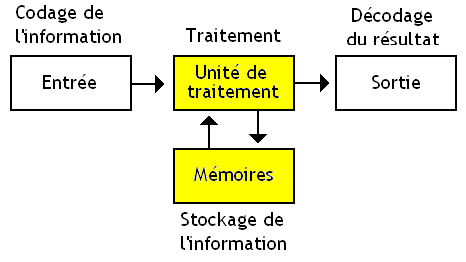
\includegraphics[trim=10 0 20 0,width=0.5\textwidth]{Images/ordinateur/Architecture_Von_Neumann_basic.png}
	\caption{Architecture d'un système à mémoire (\textit{source: https://fr.wikibooks.org/}).}
\end{figure}

\subsection{L'architecture de Von Neumann}
Jusque dans les années 40, les premiers ordinateurs étaient construits dans le but d'accomplir une tâche bien spécifique en suivant un unique programme. En 1940, le mathématicien John von Neumann imagina un type d'architecture novatrice qui permettait une programmation de la machine bien plus souple. Il eu l'idée génial d'imaginer que la mémoire pourrait servir à stocker, en plus des donnés, les instructions du programme lui même. Une telle architecture, dite de Von Neumann, décompose l’ordinateur en trois parties distinctes:
\begin{itemize}
	\item Le \textbf{processeur} qui est composé 
	\begin{itemize}
		\item d’une \textbf{unité arithmétique} et logique (UAL ou ALU en anglais) ou unité de traitement. Son rôle est d’effectuer les opérations de base (addition, multiplication, comparaison,...);
		\item  d’une \textbf{unité de contrôle} qui est chargée du séquençage des opérations du programme ;
	\end{itemize}
	\item La mémoire qui contient à la fois les données et le programme exécuté par l’unité de contrôle. La mémoire se divise entre
	 \begin{itemize}
	 	\item \textbf{mémoire vive ou RAM} (Random Access Memory) qui contient programmes et données en cours de traitement, 
	 	\item \textbf{mémoire permanente ou morte} qui stocke les programmes et données de base de la machine ;
	\end{itemize} 	
	\item Les dispositifs d’entrée-sortie, qui permettent de communiquer avec le monde extérieur.
\end{itemize}
\begin{figure}[h!]
	\centering
	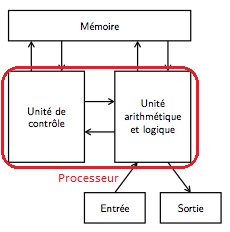
\includegraphics[trim=0 0 0 0,width=0.45\textwidth]{Images/ordinateur/arse1_archi_von_neumann_sans_accu.png}
	\caption{Architecture de Von Neumann (\textit{source: https://fr.wikibooks.org/}).}
\end{figure}

La circulation de l’information entre ces différents éléments (représentée par des flèches sur le schéma ci-dessus) est assurée par des connexions appelées \textbf{bus} (bus de données, bus d’adresse, bus de signal lecture/écriture...). Il s’agit tout simplement de fils électriques utilisés pour transmettre de données binaires.
\begin{mydefinition}
	Un \textbf{bus} informatique désigne l'ensemble des lignes de communication connectant les différents composants d'un ordinateur.
\end{mydefinition}


\subsection{Le processeur}
Le processeur, (ou CPU, Central Processing Unit, "Unité centrale de traitement" en français) est le composant essentiel d’un ordinateur qui interprète les instructions et traite les données d’un programme.
Le processeur est un circuit électronique complexe (circuit intégré) qui exécute chaque instruction très rapidement, en quelques cycles d’horloges. Toute l’activité de l’ordinateur est cadencée par une horloge unique, de façon à ce que tous les circuits électroniques travaillent tous ensemble de façon synchronisée. La fréquence de
cette horloge s’exprime en MHz (millions de cyles par seconde) ou GHz (milliards de cycles par secondes). 
\begin{important}
	Le processeur dispose d'une \textbf{horloge} (clock en anglais)  qui cadence l'exécution des instructions. L'unité est appelée \textbf{cycle}. La vitesse de cette horloge ce mesure en Hz, c'est-à-dire en nombre d'instructions exécutées en une seconde. La vitesse de l'horloge est une des caractéristiques principales pour mesurer la performance d'un processeur.
\end{important}

\begin{myexamples}
	\item le processeur de l'Iphone 13, le “Apple A13 Bionic" possède une horloge cadencée à 2,65 GHz, c'est-à-dire 2,65 milliards d'opérations par seconde.
	\item le processeur qui équipe la dernière génération de HP G4 (les PCs de la salle de cours) sont des Intel Xeon W-2225, des processeurs avec une horloge cadencée à 4,10 GHz, c'est-à-dire 4'100'000'000 opérations par seconde. 
\end{myexamples}
	
\begin{eclairage}
	Jusqu'en 2004 environ, la fréquences des ordinateurs a augmenté de manière exponentielle. Depuis elle stagne. En effet, au-delà d'une certaine fréquence il devient très difficile de dissiper la chaleur produite par le processeur ce qui perturbe la lecture des signaux électriques lus aux bornes du processeur voire détériorer le circuit électrique eu même.
	\begin{center}
		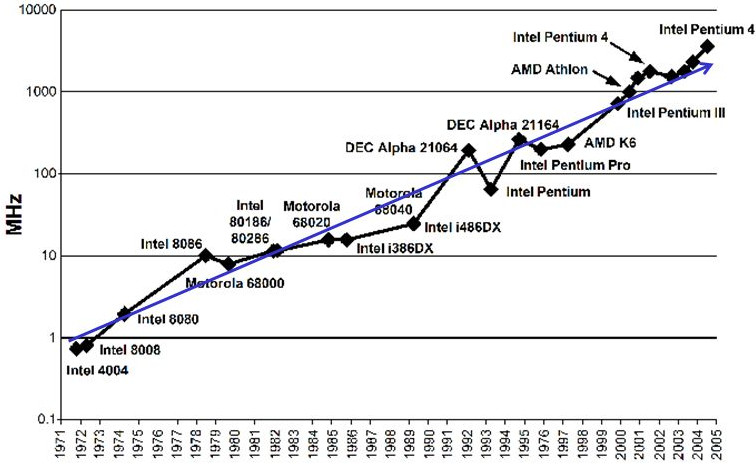
\includegraphics[trim=0 0 0 0,width=0.6\textwidth]{Images/ordinateur/evolution_frequence_ordinateur.jpg}
	\end{center}
\end{eclairage}
Pour chaque instruction,  le processeur effectue schématiquement (de manière simplifié) les opérations suivantes :
\begin{enumerate}
	\item lire dans la mémoire principale l’instruction à exécuter ;
	\item effectuer le traitement correspondant à cette instruction ;
	\item passer à l’instruction suivante.
\end{enumerate}
\begin{eclairage}
	L'architecture de Von Neumann décrit le fonctionnement de base d'un ordinateur mais c'est une simplification.  comparé celle des ordinateurs d'aujourd'hui. Par exemple,
	\begin{itemize}
		\item les entrées et sorties, initialement commandées par l’unité de contrôle du processeur, sont le plus souvent sous le contrôle (du moins partiellement) de processeurs autonomes. C’est le cas par exemple des cartes graphiques chargées de produire une image sur un écran ou des cartes sons;
		\item les ordinateurs comportent maintenant des processeurs multiples, qu’il s’agisse d’unité séparées ou de
		« cœurs » multiples à l’intérieur d’une même puce. Cette organisation permet d’atteindre une puissance
		globale de calcul élevée sans augmenter la vitesse des processeurs, limitée par les capacités d’évacuation
		de la chaleur.
	\end{itemize}	
\end{eclairage}

\newpage
\subsection{Mémoire}
\begin{wrapfigure}[]{r}{0.4\textwidth}
	\centering
	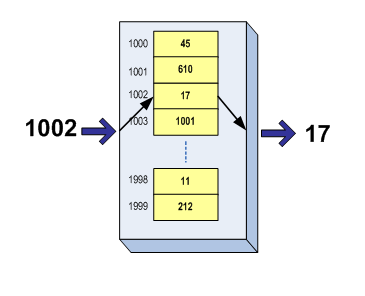
\includegraphics[trim=0 0 0 0,width=0.45\textwidth]{Images/ordinateur/adressage_memoire.png}
	\caption{Accès à la donnée "17" qui se trouve à l'adresse "1002" de la mémoire. (\textit{source: https://fr.wikibooks.org/}).}
\end{wrapfigure}
La mémoire\footnote{Ici on parle de mémoires adressables. La plupart des processeurs possèdent aussi des mémoire internet très rapide qu'on appelle \textbf{mémoire cache}.} peut être vue comme un tableau dans lequel chaque cellule est numérotée par une adresse et qui permet de stocker aussi bien les données que les programmes eux-mêmes.
%\begin{figure}[h!]
%	\centering
%	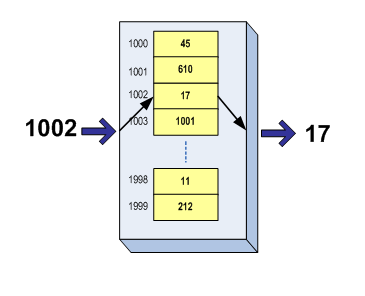
\includegraphics[trim=0 0 0 0,width=0.45\textwidth]{Images/ordinateur/adressage_memoire.png}
%	\caption{Accès à la donnée "17" qui se trouve à l'adresse "1002" de la mémoire. (\textit{source: https://fr.wikibooks.org/}).}
%\end{figure}

On distingue les mémoires en fonction de leur performance (rapidité, fiabilité, durabilité, ... ) mais surtout en fonction de leur usage:
\begin{enumerate}
	\item \textbf{La mémoire vive ou volatile} sert au stockage \textbf{temporaire} des données. Elle doit être \textbf{rapidement accessible} autant pour lire que pour stocker une donnée. En général, la technologie employée s'appuie sur des composants électroniques qui conservent les données seulement si elles sont alimentées en électricité, par conséquent, lorsque l'\textbf{ordinateur est s'éteint les données sont perdues}. \\
	\textbf{Remarque} : L'acronyme anglais RAM (Random Access Memory) est souvent utilisé pour parler de mémoire vive.
	\item \textbf{La mémoire morte} sert au stockage \textbf{persistant} des données. Lorsque l'\textbf{ordinateur est éteint les données sont conservées}.
\end{enumerate}


\begin{eclairage}
 Le processeur accède à la mémoire via des bus. Un bus est constitué d'un ensemble de fils électriques qui permettent de transmettre de l'information binaire entres plusieurs éléments de l'ordinateur. Trois bus permettent au processeur d'échanger avec la mémoire:
 \begin{enumerate}
 	\item Le \textbf{bus d'adressage} qui permet d'indiquer à la mémoire la position de la case de la mémoire qu'on souhaite accéder. Cette position est codée au moyen d'une adresse qui n'est autre qu'un nombre codé en binaire.
 	\item Le bus de données qui permet de communiquer une donnée du processeur à la mémoire (mode écriture) ou de la mémoire vers le processeur (mode lecture)
 	\item Le \textbf{bus de contrôle} qui permet, par exemple, de spécifier le mode de fonctionnement:
 		\begin{enumerate}
 			\item \textbf{mode écriture}: la donnée sur le bus est utilisé pour modifier une espace mémoire à une adresse donnée
 			\item \textbf{mode lecture}: la mémoire transmet au processeur via le bus la donnée à l'adresse demandée.
 		\end{enumerate}
 \end{enumerate}
\begin{center}
	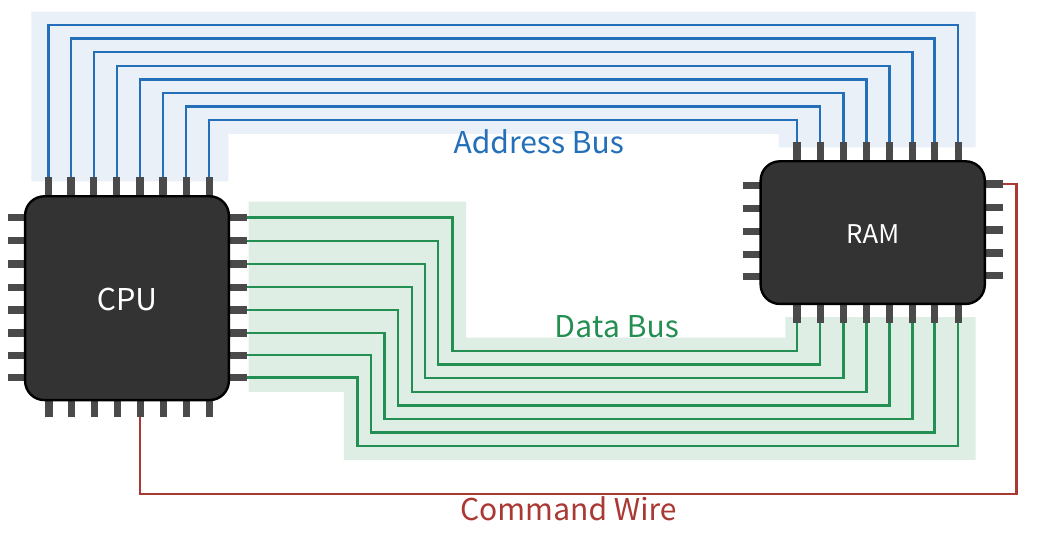
\includegraphics[trim=0 0 0 0,width=0.6\textwidth]{Images/ordinateur/cablage_memoire.png}
\end{center}
\end{eclairage}


\begin{important}
	La mémoire est principalement caractérisée par sa capacité de stockage et sa rapidité d'accès en lecture et en écriture. La capacité de stockage se mesure au nombre d'octets\footnote{Rappel: Un octet correspond à 8 bits} que la mémoire peut stocker. La vitesse se mesure en nombre d'octets par seconde qu'il est possible d'écrire ou de lire sur la mémoire.
\end{important}
\begin{myexample}
	Une clé USB de 4Go peut stocker 4 milliards d'octets, c'est à dite 32 milliards de bits.
\end{myexample}
 
\subsection{Les entrées / sorties}
Les communication avec le monde extérieur se font pas l'intermédiaire de périphérique d'entrées /sorties. Les mots entrée et sortie doivent êtres interprétés du point de vue de l'ordinateur: les entrée c'est qu'il reçoit, les sorties c'est ce qu'il renvoie.

\subsubsection{Les entrées}
L’acquisition de l’information se fait par l’intermédiaire de périphériques d’\textbf{entrées} que sont le clavier, la souris, le micro, la caméra, le scanner, l’écran tactile,... Le point commun entre tous les périphériques d'entrée est qu'ils convertissent l'information qu'ils récupèrent de l'extérieur en données compréhensibles par l'ordinateur (voir les chapitres \ref{codageNombre} et 2).

\subsubsection{Les sorties}
La restitution de l’information se fait par l’intermédiaire de périphériques de \textbf{sorite} que sont l'écran, les écouteurs, l'imprimante,... Ils décodent l'information fournie par l'ordinateur afin de la rendre compréhensible par l'utilisateur (le plus souvent sous forme de textes, images ou sons).

\section{Les ordinateurs d'aujourd'hui}
\begin{wrapfigure}[]{r}{0.45\textwidth}
	\centering
	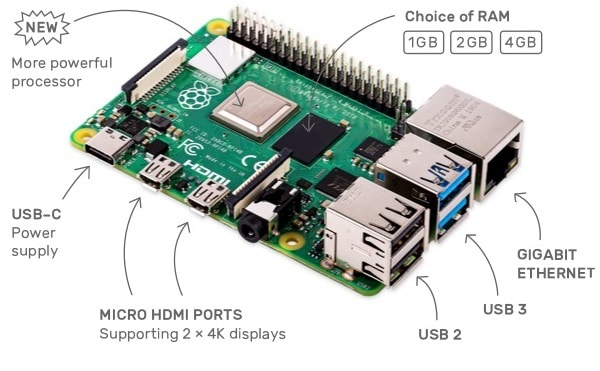
\includegraphics[trim=0 0 0 120,width=0.5\textwidth]{Images/ordinateur/raspberry-pi-4-caracteristiques.jpg}
	\caption{\small Un RaspberryPi 4 .}
\end{wrapfigure}
Nous sommes entouré d'ordinateurs. Par exemple, aujourd'hui vous avez sûrement consulté les écrans d'affichage du collège qui fonctionnent avec un \textbf{Raspberry Pi} (qui est nano-ordinateur monocarte) en se connectant sur un serveur internet. Vous avez aussi probablement consulté votre smartphone (l'ordinateur le plus populaire du monde \footnote{ \url{https://www.numerama.com/tech/722898-le-smartphone-est-lordinateur-le-plus-populaire-au-monde.html}})
et finalement vous allez utiliser un PC (Personnal Computer), ou ordinateur personnel, pendant le cours d'informatique.
\newpage

\section{Le PC}
Le terme \textbf{PC} (Personnal Computer) ou ordinateur personnel désigne un ordinateur qui répond aux besoins des utilisateurs humains et qui est de dimension raisonnable, c'est-à-dire qu'il peut tenir sur un bureau. On parle aussi de micro-ordinateur ou ordinateur individuel. 



\subsection{Les composants  d'un PC}
La carte mère (1) qui est le circuit imprimé \footnote{Le circuit imprimé est un support, en général une plaque, permettant de maintenir et de relier électriquement un ensemble de composants électroniques entre eux.} qui supporte et relie tous les composants propres et les périphériques propres de l'ordinateur. Elle permet de prendre en charge la mémoire vive (4), la lecture du disque dur (7) et l'utilisation du processeur. Cette carte mère est fixée à l'unité centrale également nommée : la tour, le boîtier, desktop, etc.

\begin{center}
	\begin{figure}[h]
		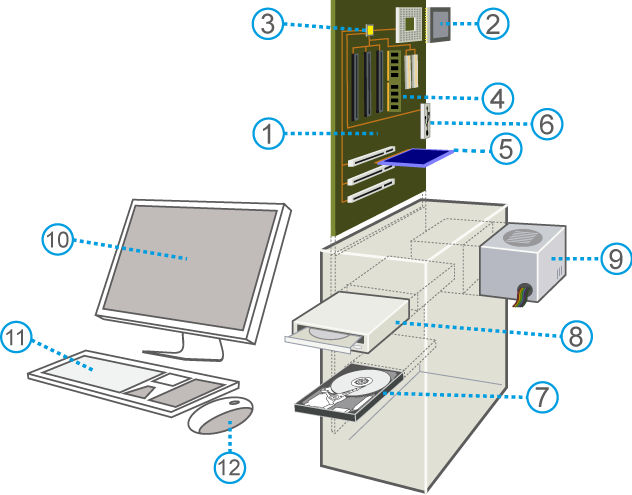
\includegraphics[scale=.6]{Images/ordinateur/composants}
		\caption{L'ordinateur, l'unité centrale et sa composition}
		\label{composants}
	\end{figure}
\end{center}

Les principaux composants constituant un ordinateur sont :
\begin{itemize}%[label=\textbullet]
	\item Le {\bf processeur} (CPU, Central Processing Unit) (2): qui est l'élément central de la carte mère.
	
	\item  La {\bf mémoire vive} (RAM) (4) : qui est sous la forme de une ou plusieurs barrettes qui se fixent à la carte mère.

	\item La {\bf mémoire permanente}: qui était le plus souvent sous la forme de disque dur optique (hard drive, 7) mais qui tend à être remplacé par des disques électronique1 de type SSD (de l'anglais \textit{solid-state drive}).
	
	\item  Le {\bf lecteur/graveur CD/DVD/Blu-ray } (8) : qui il lit l'ensemble des CD, DVD et Blu-ray, que ce soit de la musique, des logiciels, des jeux, des films, etc. Son utilisation par défaut tend à disparaître.
	
	\item L'{\bf alimentation} (9) : branchée sur le réseau électrique 220 [V], elle alimente tous les composants électroniques.
	
	\item La {\bf carte graphique} (graphic card) (5) : elle transmet les images qu'elle possède en mémoire sur les écrans. Elle permet donc d'afficher à l'écran des images, du texte, des vidéos, etc. en allumant des points lumineux (pixels). À noter que certains processeurs comportent une unité graphique rendant obsolète l'ajout d'une carte graphique sur un ordinateur, typiquement pour un usage de type bureautique.
\end{itemize}


\subsection{Caractéristiques détaillés des composants}


\subsubsection{La carte mère}
\begin{wrapfigure}[]{r}{0.4\textwidth}
\centering
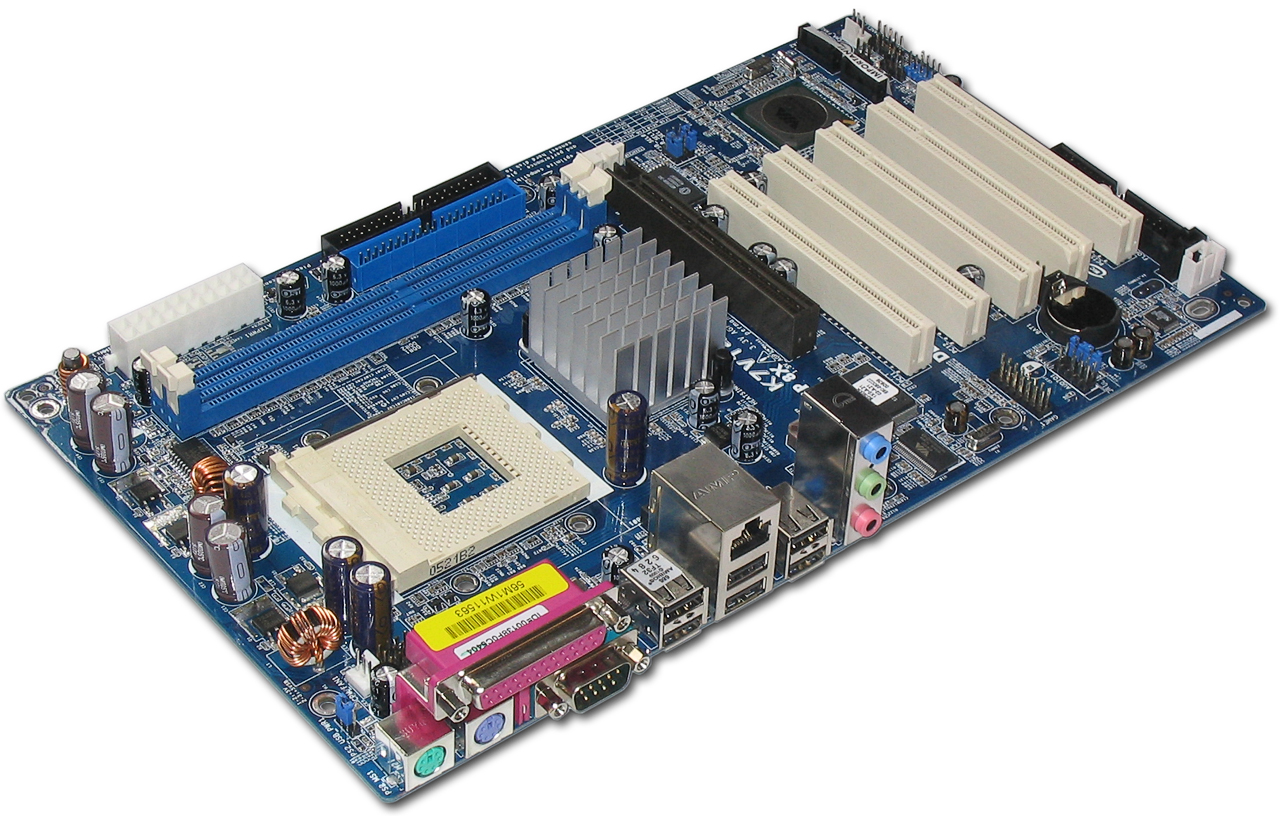
\includegraphics[trim=0 0 0 000 ,scale=.4]{Images/ordinateur/cartemere}
\caption{Carte mère d'un PC}
\end{wrapfigure}
Une {\bf carte mère} se distingue principalement par la génération de processeur qu'elle peut accueillir, par le type de mémoire vive pouvant être connecté, le nombre et les différents types de connecteurs (6) (IDE, sata, PCI, etc.) qu'elle comporte  et par son jeu de composants électroniques (chipset) lui permettant de gérer l'échange de données entre les disques, la mémoire, la carte graphique et les différents périphériques externes d'entrée/sortie. La carte mère comporte également un ensemble de fonctions nommé BIOS ({\it Basic Input Output System}) ou plus récemment UEFI ({\it Unified Extensible Firmware Interface}) lui permettant, lors de sa mise sous tension, d'identifier le matériel connecté sur la carte mère.



\subsubsection{Processeur}
\begin{wrapfigure}[]{r}{0.4\textwidth}
	\centering
	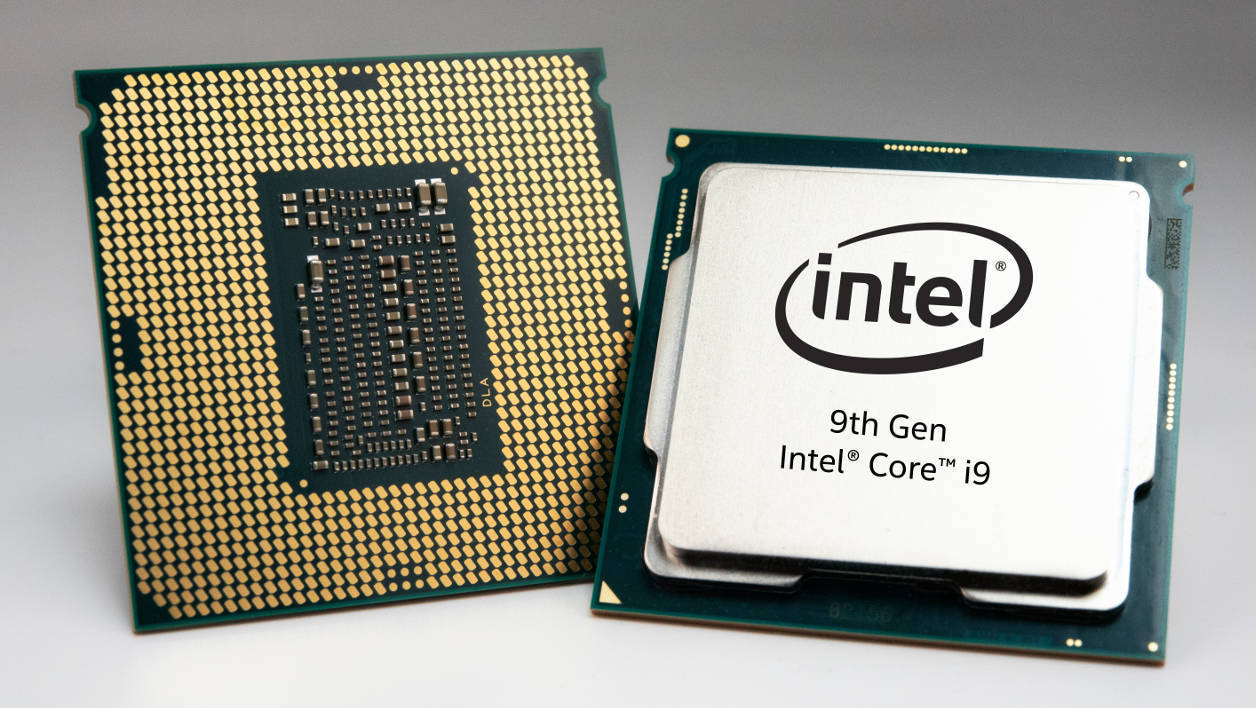
\includegraphics[trim=0 0 0 400 ,width=0.4\textwidth]{Images/ordinateur/processeur}	\caption{Un processeur Intel i9}
\end{wrapfigure}
Un processeur se distingue principalement par sa fréquence de fonctionnement et son architecture (nombre de cœurs, mémoire cache, ...). À l’heure actuelle, la fréquence des PCs varie de 2GHz à 4GHz. Les deux plus important fabricants de processeur de PCs sont Intel et AMD.


\subsubsection{Mémoire}
Qu'il s'agisse de {\bf mémoire vive (RAM)} ou {\bf mémoire permanente}, la mémoire est principalement caractérisée par sa capacité de stockage et sa rapidité d'accès en lecture et en écriture. Actuellement, sa capacité est traduite en gigaoctets [Go] ou téraoctets [To]. La vitesse de lecture et d'écriture est donnée en Mo/s (megaoctets par seconde).
%\begin{figure}[h!]
%	\centering
%	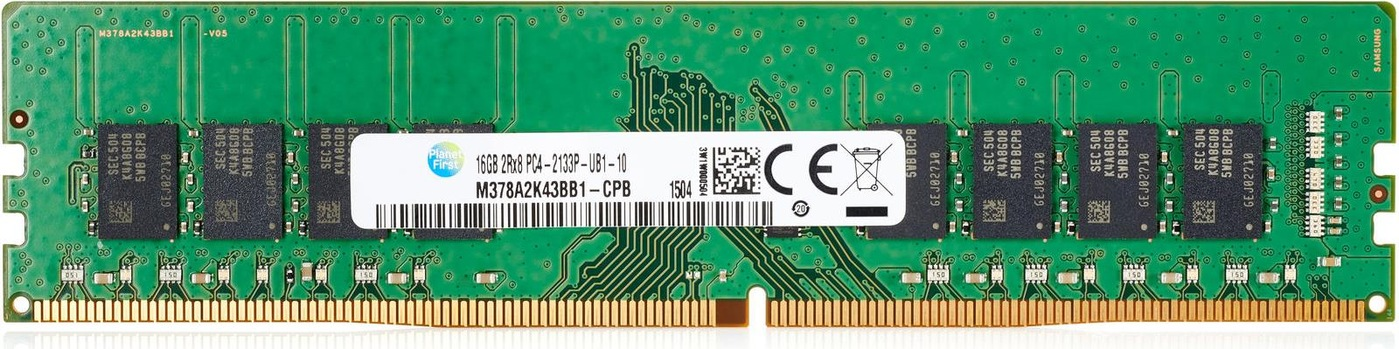
\includegraphics[scale=.2,trim=0 0 0 0]{Images/ordinateur/sdram.jpg}
%	\caption{barrette de RAM}
%\end{figure}
\begin{figure}[h!]
	\centering
	\subfloat[barrette de RAM]{%
		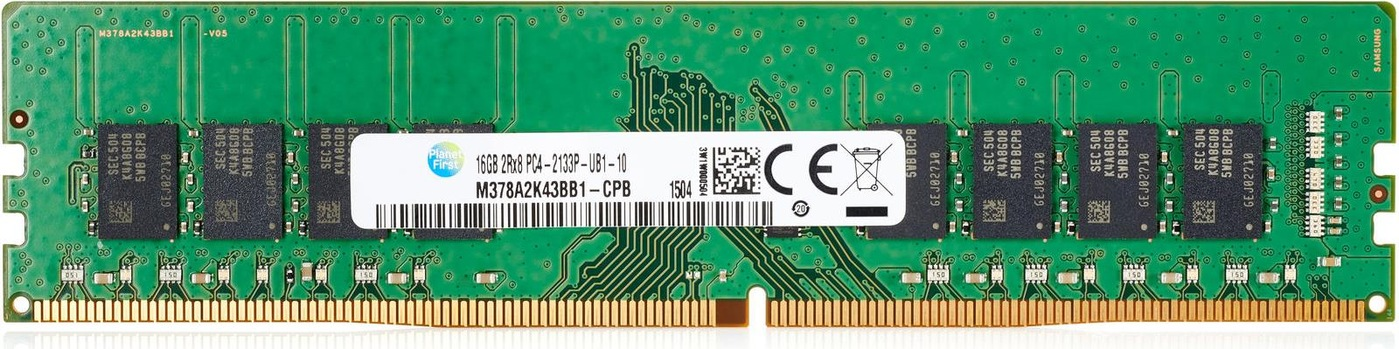
\includegraphics[width=0.5\textwidth,trim=0 0 0 60]{Images/ordinateur/sdram.jpg}
	}
	\hspace{1cm}
	\subfloat[Disque dur]{%
		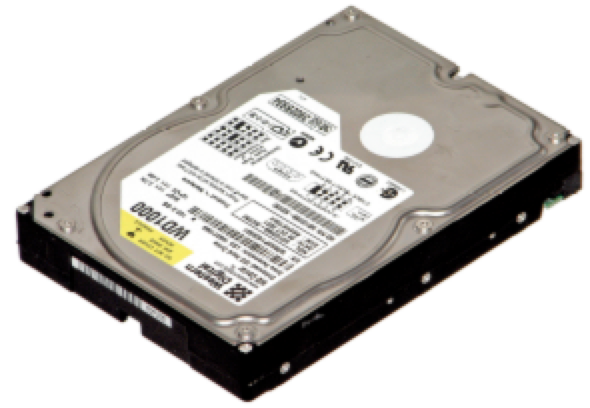
\includegraphics[width=0.3\textwidth,trim=0 0 0 60]{Images/ordinateur/disquedur}
	}
	\caption{Mémoire vive et morte.}
	\label{img_coul}
\end{figure}

\subsubsection{La carte graphique}
\begin{wrapfigure}[]{r}{0.4\textwidth}
	\centering
	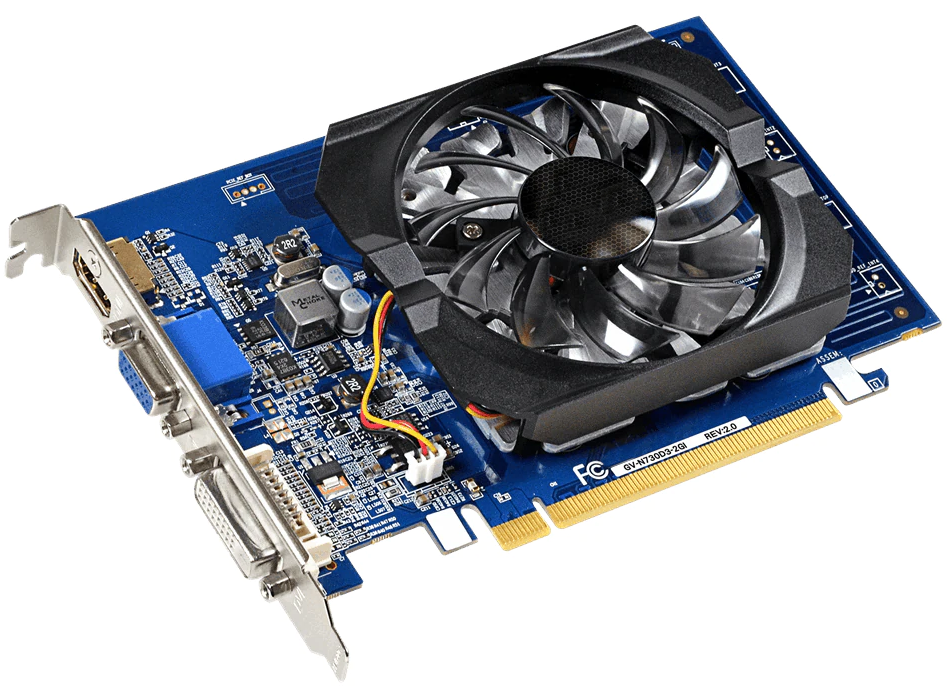
\includegraphics[scale=.2,trim=0 0 0 200]{Images/ordinateur/carte_graphique}
\end{wrapfigure}
La {\bf carte graphique} se caractérise principalement par l'architecture de son processeur graphique (GPU) et sa mémoire vive. À ce jour, Nvidia et AMD sont leaders dans la conception des processeurs graphiques. On distingue très facilement les cartes graphiques les plus puissantes par le système de refroidissement qu’elle possède.





\section{Périphériques externes}

\subsection{Exemples de périphériques}

Pour interagir avec l’ordinateur, des périphériques d’entrée/sortie sont nécessaires. Il en existe de toutes sortes et ces derniers sont connectés à l’ordinateur par différent type de câbles (réseau, USB, DVI, série, etc.) ou à l’aide d’une connexion sans fils (infrarouge, wifi, Bluetooth, lasers, etc).

\begin{figure}[h]
	\centering
	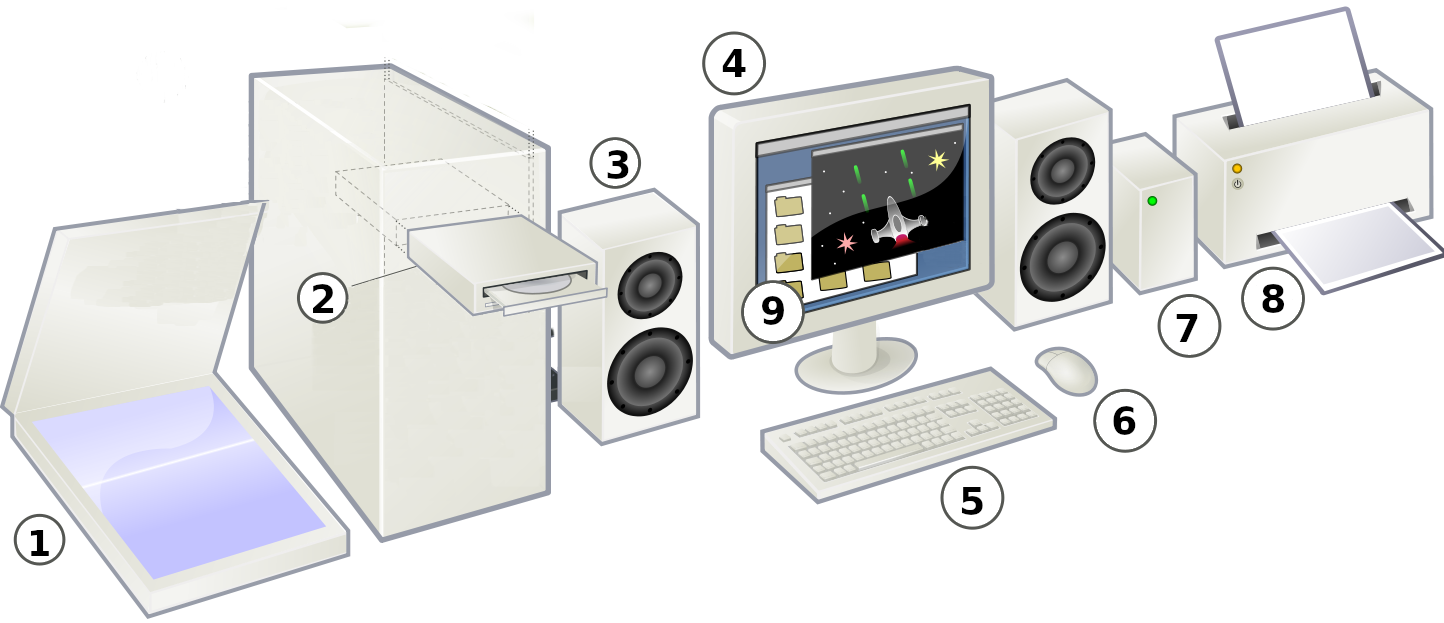
\includegraphics[scale=.3]{Images/ordinateur/peripherique}
	\caption{Périphériques d'un ordinateur}
\end{figure}


Les différents types de périphériques externes sont :
\begin{enumerate}
	\item Le {\bf scanner} permet la numérisation de document dans une certaine résolution.
	\item Le {\bf lecteur} CD ou DVD ou Blu-ray sont des lecteurs permettant de lire un support amovible à l’aide d’un faisceau laser.
	\item Le {\bf haut-parleur} permet de diffuser du son.
	\item L’{\bf écran} permet d’afficher les informations, mais lorsqu’il est tactile, il offre la possibilité de se passer de la souris et du clavier. Il est caractérisé par sa taille et sa définition1 d’écran qui est le nombre de points ou pixels que peut afficher un écran. Actuellement, les définitions (nombre de points H x V) les plus courantes sur un écran pour ordinateur sont :
	\begin{itemize}
		\item XGA : 1024 x 768
		\item  HD : 1280 x 768
		\item  Full HD : 1920 x 1080
		\item WUXGA : 1920 x 1200
		\item  WQHD : 2560 x 1440
		\item 8K Full Format : 8192 x 4320
	\end{itemize}
	\item le {\bf clavier} utilisé pour écrire, mais également se déplacer rapidement dans un texte ou dans des menus voir même effectuer une copie d’écran (screenshot).
	\item La {\bf souris} sert à déplacer le curseur sur l’écran, de choisir des applications et aussi de cliquer sur des icônes pour démarrer des logiciels. Elle permet de naviguer sur votre ordinateur, mais également de dessiner, sélectionner des textes, etc. Elle est mobile avec ou sans fil.
	\item Le {\bf disque externe} est un disque dur qui n’est pas intégré dans l’ordinateur. En fonction de sa taille, il peut être facilement déplacé. En fonction du modèle, les disques externes sont soit alimentés par un branchement USB, soit avec une alimentation sur secteur 220[V].
	\item L’{\bf imprimante} 2D permet l’impression de texte, image, graphique. Il existe plusieurs technologies d’impressions telles que laser, jet d’encre, sublimation, etc. Depuis les années 2010, l’impression 3D prend de l’ampleur avec l’arrivée de nouvelles technologies innovantes basées sur de nouveaux matériaux comme le plastique, la cire, le métal, la céramique, le verre. Il est même possible d’imprimer en 3D une forme en chocolat !
	\item L’{\bf interface graphique} ou l’{\bf environnement graphique} est un dispositif logiciel permettant le dialogue entre l’utilisateur·trice et l’ordinateur.
	En fonction de son utilisation, un périphérique est considéré soit en entrée, soit en sortie, soit comme étant bidirectionnel. Le tableau suivant résume le type de périphérique.
\end{enumerate}

En fonction de son utilisation, un périphérique est considéré soit en entrée, soit en sortie, soit comme étant bidirectionnel. Le tableau suivant résume le type de périphérique.
\begin{center}
	\begin{tabular}{|l|c|c|}
		\hline
		\textbf{Périphériques externes}                                                                                                                   & \multicolumn{1}{l|}{\textbf{\begin{tabular}[c]{@{}l@{}}Périphérique\\ d’entrée\end{tabular}}} & \multicolumn{1}{l|}{\begin{tabular}[c]{@{}l@{}}Périphérique \\ de sortie\end{tabular}} \\ \hline
		\begin{tabular}[c]{@{}l@{}}Souris, clavier, caméra internet  (webcam),  scanner \\ 2D et 3D, lecteur (CD, DVD, Blu-ray), microphone.\end{tabular} & x                                                                                             &                                                                                        \\ \hline
		Écran, haut-parleur, imprimante 2D et 3D                                                                                                          &                                                                                               & x                                                                                      \\ \hline
		\begin{tabular}[c]{@{}l@{}}Écran tactile (touch screen), disque dur externe,\\ graveur (CD, DVD, Blu-ray).\end{tabular}                           & x                                                                                             & x                                                                                      \\ \hline
	\end{tabular}
\end{center}

\newpage

\section{Le smartphone}
Les smartphone sont aussi des ordinateur qui possède des périphériques d'entrée :
\begin{itemize}
	\item Un microphone (4),
	\item Une antenne (6) pour emmètre des données sur le réseau,
	\item Une caméra pour prendre des photos/vidéos,
	\item accéléromètre 6 axes,
	\item un puce GPS pour déterminer les coordonnées de l'appareil sur la terre,
\end{itemize}
des périphériques de sortie :
\begin{itemize}
	\item Un haut-parleur (7),
\end{itemize}
ainsi que des périférique mixtes, qui sont d'entrée et de sortie: 
\begin{itemize}
	\item Une antenne GMS (6) pour recevoir et envoyer des données sur le réseau téléphonique,
	\item Un écran tactile (2) qui permet d'afficher des informations et à l'utilisateur d'interagir avec le téléphone,
	\item  un module bluetooth et wifi qui permettent de transférer des données en utilisant des deux types de réseaux.
\end{itemize}

\begin{figure}[h!]
	\centering
	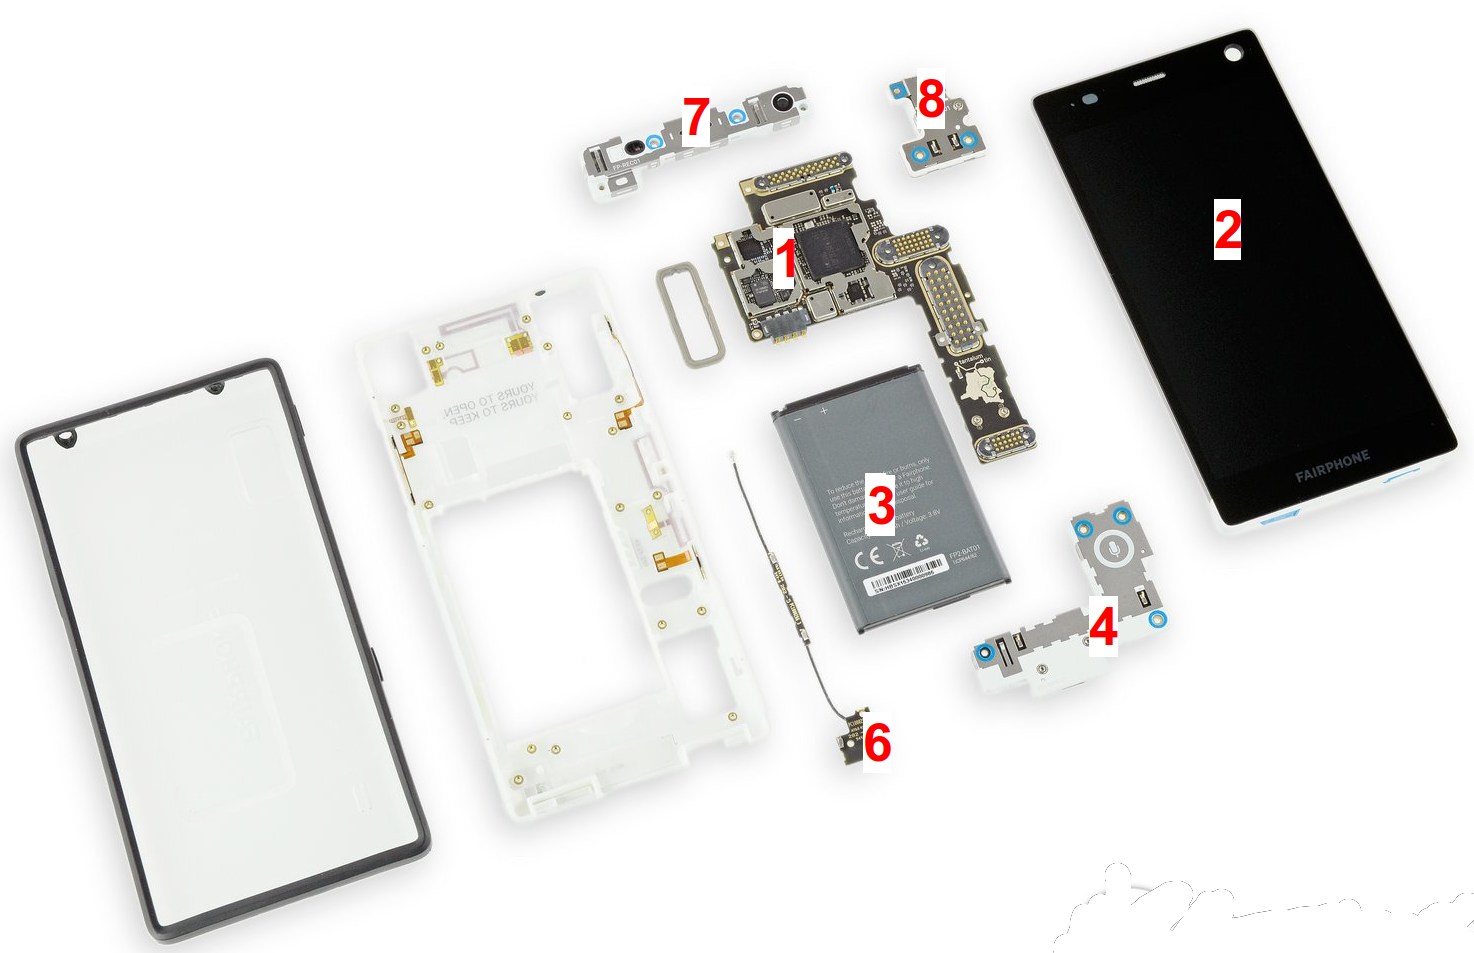
\includegraphics[width=0.9\textwidth]{Images/ordinateur/fairphone}
	\caption{Exemple d'un Fairphone 2. Le téléphone est facilement réparable, chaque composant peut être démonté.}
\end{figure}

Le téléphone est alimenté par une batterie (3). Sur la carte mère (1) on retrouve le processeur (8) qui est superposé à la mémoire (RAM), ainsi qu'une mémoire flash (9) qui fait office de mémoire persistante. 
\begin{figure}[h!]
	\centering
	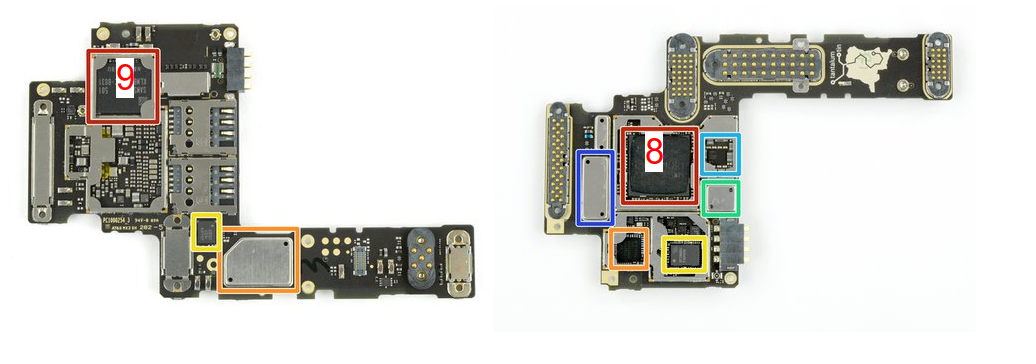
\includegraphics[width=0.9\textwidth]{Images/ordinateur/fairphoneCarteMere.png}
	\caption{Les deux face de la carte mère d'un Fairphone 2.}
\end{figure}

\begin{eclairage}
	Afin de diminuer la dimension des smartphone, c'est souvent le {\bf SoC, (system on a chip)} qui rassemble quasiment tous ces composants: CPU, GPU (processeur de la carte graphique), modem (connexion réseau), mémoire RAM... Dans une petite puce (M1 ou A11 par exemple chez apple ou Exynos chez Samsung) se retrouve concentré la puissance d'un ordinateur d'il y a quelques années.
\end{eclairage}
	

\section{Les serveurs}
Il existe des ordinateurs plus puissants qui sont spécialement conçus pour fournir des informations et des logiciels à d'autres ordinateurs reliés via un réseau. On les appelle des {\bf serveurs}. Ces derniers sont capables de traiter des charges de travail plus importantes et d'exécuter davantage d'applications.

\begin{figure}[h]
	\centering
	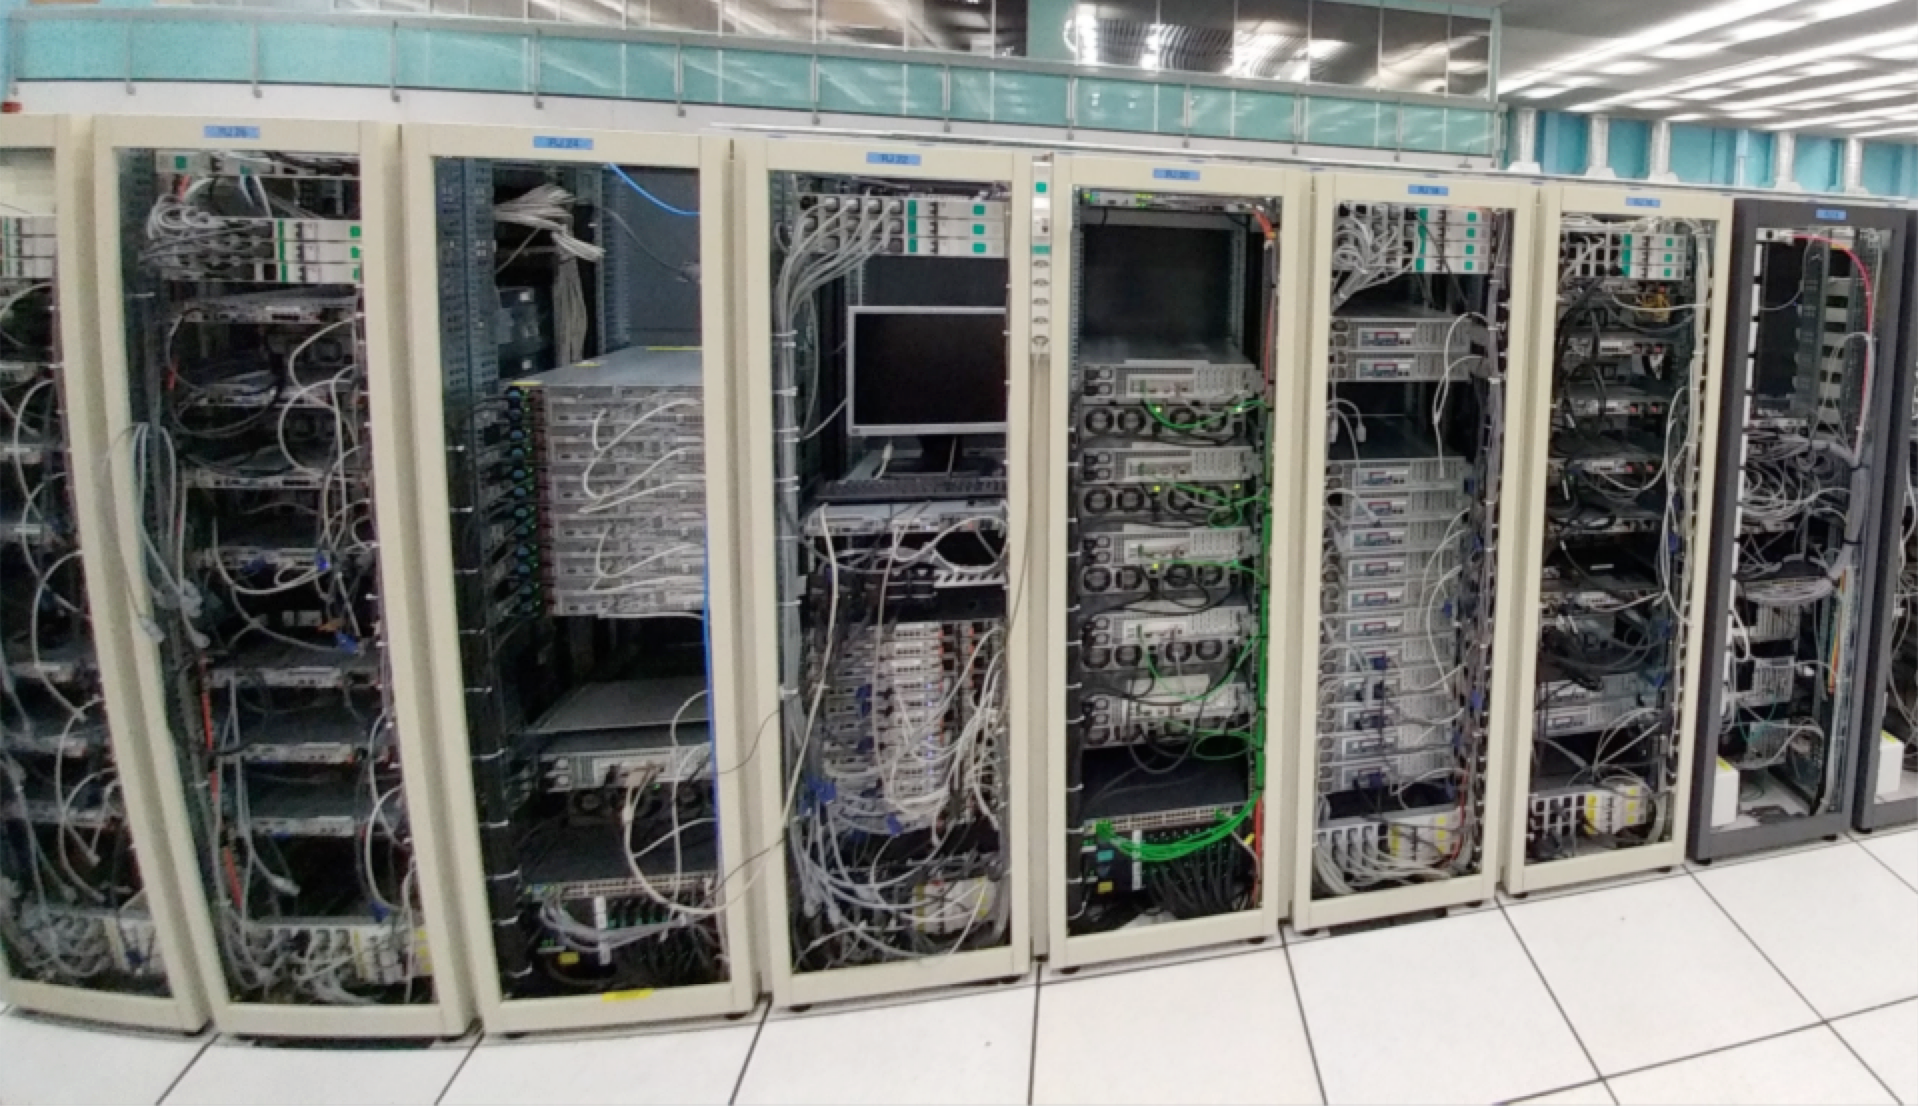
\includegraphics[scale=.4]{Images/ordinateur/serveur}
	\caption{Salle de serveurs du CERN}
	\label{serveur}
\end{figure}


Les ordinateurs les plus puissants au monde sont appelés supercalculateur. Ils contiennent des centaines, voire des milliers de processeurs. Ils sont souvent utilisés dans la recherche médicale, les applications scientifiques (cf Figure \ref{serveur}), le domaine de la finance, la météorologie et à des fins militaires.

